\documentclass[a4paper,11pt]{article}

% --- Packages ---
\usepackage[margin=1in]{geometry}
\usepackage{amsmath, amssymb}
\usepackage{booktabs}
\usepackage{graphicx}
\usepackage{enumitem}
\usepackage{hyperref}
\usepackage{xcolor}
\usepackage{tikz}
\usepackage{pgfplots}
\pgfplotsset{compat=1.18}

% --- Styling helpers ---
\setlist[itemize]{left=1.2em,itemsep=0.25em,topsep=0.25em}
\newcommand{\exline}{\vspace{0.35em}\hrule\vspace{0.6em}}

% Metric block macro: title, formula, meaning, example (left-aligned)
\newcommand{\metric}[4]{%
\subsection*{#1}
\[
#2
\]
\noindent\textbf{Meaning:} #3

\vspace{0.8em}

\noindent\textbf{Example:} #4

\exline
}

% --- Title page ---
\title{\vspace{-2cm}\textbf{\LARGE Binary Classification Metrics Cheat Sheet}}
\author{\textbf{ROSCODE TECH}\\[0.25em]\small roscoekerby}
\date{\today}

\begin{document}
\maketitle
\thispagestyle{empty}
\vfill
\begin{center}
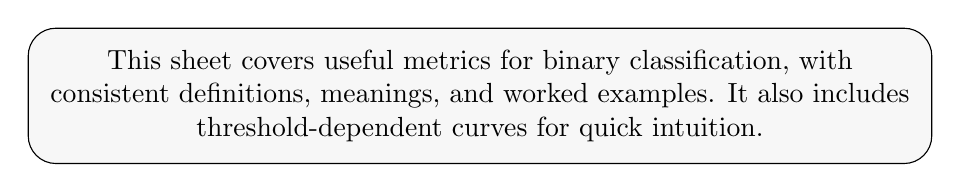
\begin{tikzpicture}
\node[draw, rounded corners=10pt, inner sep=8pt, fill=black!3] (box) {
\begin{minipage}{0.9\linewidth}
\centering
This sheet covers useful metrics for binary classification, with consistent definitions, meanings, and worked examples. It also includes threshold-dependent curves for quick intuition.
\end{minipage}};
\end{tikzpicture}
\end{center}
\vfill
\newpage

\tableofcontents
\newpage

\section{Confusion Matrix and Notation}

\begin{center}
\renewcommand{\arraystretch}{1.25}
\begin{tabular}{@{}lcc@{}}
\toprule
 & \textbf{Predicted Positive} & \textbf{Predicted Negative} \\
\midrule
\textbf{Actual Positive} & True Positive (TP) & False Negative (FN) \\
\textbf{Actual Negative} & False Positive (FP) & True Negative (TN) \\
\bottomrule
\end{tabular}
\end{center}

\noindent Total samples: \(N = TP + TN + FP + FN\).

\paragraph{Running example.}
Unless stated otherwise, use: \(TP=50\), \(FN=10\), \(FP=5\), \(TN=35\), so \(N=100\).

\exline

\section{Core Metrics}

\metric{Accuracy}{\displaystyle Accuracy=\frac{TP+TN}{N}}{Fraction of all predictions that are correct.}{\(\frac{50+35}{100}=0.85\).}

\metric{Sensitivity, Recall, True Positive Rate (TPR)}{\displaystyle Recall=\frac{TP}{TP+FN}}{Ability to find actual positives.}{\(\frac{50}{50+10}=0.83\).}

\metric{Specificity, True Negative Rate (TNR)}{\displaystyle Specificity=\frac{TN}{TN+FP}}{Ability to correctly reject actual negatives.}{\(\frac{35}{35+5}=0.875\).}

\metric{Precision, Positive Predictive Value (PPV)}{\displaystyle Precision=\frac{TP}{TP+FP}}{Reliability of positive predictions.}{\(\frac{50}{50+5}=0.91\).}

\metric{Negative Predictive Value (NPV)}{\displaystyle NPV=\frac{TN}{TN+FN}}{Reliability of negative predictions.}{\(\frac{35}{35+10}=0.78\).}

\metric{F1 Score}{\displaystyle F1=\frac{2\,(\text{Precision}\cdot \text{Recall})}{\text{Precision}+\text{Recall}}}{Harmonic mean of precision and recall. Encourages balance.}{With Precision \(=0.91\) and Recall \(=0.83\): \(F1=\frac{2\cdot 0.91\cdot 0.83}{0.91+0.83}\approx 0.87\).}

\metric{Balanced Accuracy}{\displaystyle \text{Balanced Accuracy}=\tfrac{1}{2}\left(\text{Recall}+\text{Specificity}\right)}{Equal weight for positive and negative classes. Useful with imbalance.}{\(\tfrac{1}{2}(0.83+0.875)=0.8525\).}

\metric{Error Rates (FPR, FNR)}{\displaystyle FPR=\frac{FP}{FP+TN},\qquad FNR=\frac{FN}{TP+FN}}{FPR is the false alarm rate on negatives. FNR is the miss rate on positives.}{\(FPR=\frac{5}{40}=0.125\), \(FNR=\frac{10}{60}\approx 0.167\).}

\metric{Matthews Correlation Coefficient (MCC)}{\displaystyle MCC=\frac{TP\cdot TN-FP\cdot FN}{\sqrt{(TP+FP)(TP+FN)(TN+FP)(TN+FN)}}}{Correlation between prediction and truth. Robust under class imbalance.}{\(\frac{50\cdot 35-5\cdot 10}{\sqrt{55\cdot 60\cdot 40\cdot 45}}\approx 0.74\).}

\metric{Cohen's Kappa}{\displaystyle
\kappa=\frac{p_o-p_e}{1-p_e},\quad
p_o=\frac{TP+TN}{N},\quad
p_e=\frac{(TP{+}FN)(TP{+}FP)+(TN{+}FP)(TN{+}FN)}{N^2}
}{Agreement beyond chance.}{\(p_o=0.85\), \(p_e=\frac{3300+1800}{10000}=0.51\), so \(\kappa=\frac{0.85-0.51}{1-0.51}=0.69\).}

\metric{Youden's \(J\)}{\displaystyle J=\text{Sensitivity}+\text{Specificity}-1}{Single summary of informedness.}{\(0.83+0.875-1=0.705\).}

\metric{Geometric Mean (G-Mean)}{\displaystyle G\text{-}Mean=\sqrt{\text{Sensitivity}\cdot \text{Specificity}}}{Balance between catching positives and rejecting negatives.}{\(\sqrt{0.83\cdot 0.875}\approx 0.852\).}

\exline

\section{Calibration Metrics}

\metric{Log Loss (Cross Entropy)}{\displaystyle \text{LogLoss}=-\frac{1}{N}\sum_{i=1}^{N}\Big[y_i\log(p_i)+(1-y_i)\log(1-p_i)\Big]}{How well predicted probabilities match outcomes. Lower is better.}{If a positive is predicted with \(p=0.9\), contribution is \(-\log(0.9)=0.105\). If it was actually negative, contribution would be \(-\log(1-0.9)=2.303\).}

\metric{Brier Score}{\displaystyle \text{Brier}=\frac{1}{N}\sum_{i=1}^N (p_i-y_i)^2}{Mean squared error of predicted probabilities. Lower is better.}{For three cases with \((p,y)=(0.8,1),(0.4,0),(0.3,1)\): score \(=\frac{(0.2)^2+(0.4)^2+(0.7)^2}{3}\approx 0.203\).}

\exline

\section{Threshold Curves}

\subsection*{ROC Curve and AUC}
\textbf{Formula.} Plot \(TPR=\frac{TP}{TP+FN}\) against \(FPR=\frac{FP}{FP+TN}\) while sweeping the decision threshold from 1 to 0.  
\textbf{Meaning.} Trade-off between sensitivity and false alarms.  
\textbf{Example.} At threshold \(0.50\): \(TPR=0.83\), \(FPR=0.125\).

\begin{center}
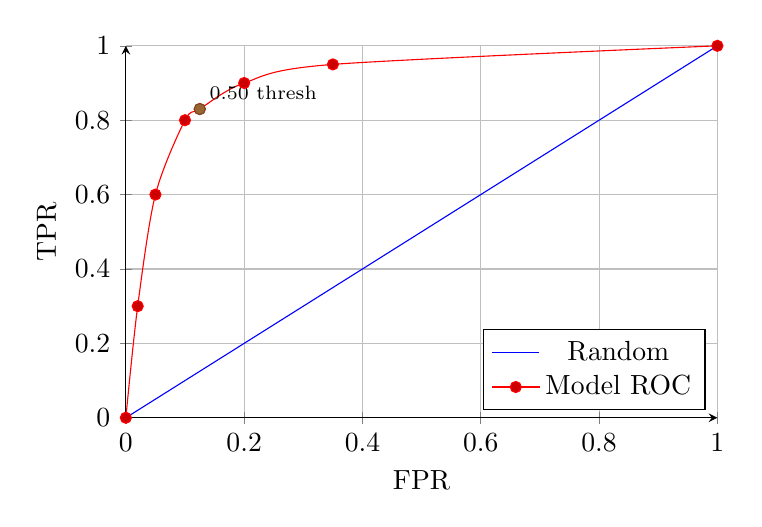
\begin{tikzpicture}
\begin{axis}[
    width=0.75\linewidth,
    height=0.52\linewidth,
    xlabel={FPR},
    ylabel={TPR},
    xmin=0,xmax=1,ymin=0,ymax=1,
    axis lines=left,
    grid=both,
    ticks=both,
    legend style={at={(0.98,0.02)},anchor=south east}
]
% Random baseline
\addplot+[mark=none,domain=0:1,samples=2] {x}; \addlegendentry{Random}
% Example ROC curve (monotone increasing, step-like)
\addplot+[mark=*, smooth] coordinates {
(0.00,0.00)
(0.02,0.30)
(0.05,0.60)
(0.10,0.80)
(0.125,0.83)
(0.20,0.90)
(0.35,0.95)
(1.00,1.00)
}; \addlegendentry{Model ROC}
% Annotate the 0.50 threshold point
\addplot+[only marks, mark=*] coordinates {(0.125,0.83)};
\node[anchor=south west] at (axis cs:0.125,0.83) {\scriptsize 0.50 thresh};
\end{axis}
\end{tikzpicture}
\end{center}

\subsection*{Precision–Recall Curve}
\textbf{Formula.} Plot Precision \(=\frac{TP}{TP+FP}\) versus Recall \(=\frac{TP}{TP+FN}\) across thresholds.  
\textbf{Meaning.} Often more informative than ROC when positives are rare.  
\textbf{Example.} At threshold \(0.50\): Precision \(=0.91\), Recall \(=0.83\).

\begin{center}
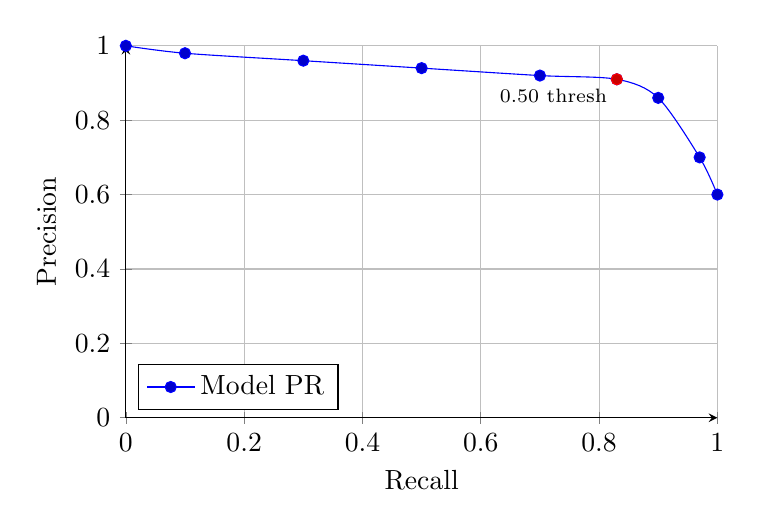
\begin{tikzpicture}
\begin{axis}[
    width=0.75\linewidth,
    height=0.52\linewidth,
    xlabel={Recall},
    ylabel={Precision},
    xmin=0,xmax=1,ymin=0,ymax=1,
    axis lines=left,
    grid=both,
    ticks=both,
    legend style={at={(0.02,0.02)},anchor=south west}
]
% A plausible PR curve that stays high then decays
\addplot+[mark=*, smooth] coordinates {
(0.00,1.00)
(0.10,0.98)
(0.30,0.96)
(0.50,0.94)
(0.70,0.92)
(0.83,0.91)
(0.90,0.86)
(0.97,0.70)
(1.00,0.60)
}; \addlegendentry{Model PR}
% Highlight the 0.50 threshold point
\addplot+[only marks, mark=*] coordinates {(0.83,0.91)};
\node[anchor=north east] at (axis cs:0.83,0.91) {\scriptsize 0.50 thresh};
\end{axis}
\end{tikzpicture}
\end{center}

\exline

\section{Quick Tips}
\begin{itemize}
  \item Use Balanced Accuracy, MCC, F1, and PR curves when classes are imbalanced.
  \item Move the threshold to trade precision for recall, or the reverse. Choose based on the application cost.
  \item F1 ignores true negatives. If true negatives matter, consider MCC or Balanced Accuracy.
  \item AUC is threshold independent, yet PR curves can be more revealing when positives are rare.
  \item Check calibration with Log Loss or Brier before using probabilities downstream.
\end{itemize}

\end{document}
